\documentclass{beamer}
\usepackage[utf8]{inputenc}
\usepackage{graphicx, epsfig}
\usepackage{amsmath,mathrsfs,amsfonts,amssymb}
\usepackage{subfigure}
\usepackage{floatflt}
\usepackage{epic,ecltree}
\usepackage{mathtext}
\usepackage{fancybox}
\usepackage{xcolor}
\usepackage{fancyhdr}
\usepackage{bm}
\usepackage{multirow}
\usepackage{enumerate}
\usepackage{epstopdf}
\usepackage{multicol}
\usetheme{Copenhagen}%{Singapore}%{Warsaw}%{Warsaw}%{Darmstadt}
\usecolortheme{whale}
%\definecolor{beamer@blendedblue}{RGB}{15,120,80}
\definecolor{orangemy}{RGB}{66, 138, 183}
\newcommand{\T}{{\text{\tiny\sffamily\upshape\mdseries T}}}
\DeclareMathOperator*{\argmax}{arg\,max}
%--------------------------------------------------------------------------------
\title[\hbox to 56mm{Bayesian Neural Networks  \hfill\insertframenumber\,/\,\inserttotalframenumber}]
{Bayesian Neural Networks}
\author[ROY team]{\\
	{\small \textbf{ROY team:} Ilya Zharikov, \\ \hspace{2.67cm}Roman Isachenko, \\ \hspace{2.61cm}Artem Bochkarev}}
\institute[SkolTech]{Skolkovo Institute of Science and Technology \\
	Bayesian Methods course 
	\vspace{0.3cm}
}
\date{May 25, 2017}
%--------------------------------------------------------------------------------
\begin{document}
	%--------------------------------------------------------------------------------
	\begin{frame}
		%\thispagestyle{empty}
		\titlepage
	\end{frame}
%--------------------------------------------------------------------------------
\begin{frame}{Project goal}	
	\begin{block}{Goal}
		Estimate posterior distributions of the model parameters from data
	\end{block}
	\begin{block}{Problem}
		Monte Carlo sampling is very slow for high-dimensional data
	\end{block}	

	\vfill

	\textbf{Probabilistic Programming:}
	\begin{itemize}
		\item Uncertainty in predictions;
		\item Uncertainty in representations;
		\item Regularizations with priors;
		\item Transfer learning;
		\item Hierarchical Neural Networks.
	\end{itemize}
\end{frame}
%--------------------------------------------------------------------------------
\begin{frame}{Related work}
	\begin{enumerate}
		\item Salvatier J, Wiecki T.\,V., Fonnesbeck C. Probabilistic programming in Python using PyMC3. // \emph{PeerJ Computer Science}. 2016.
		\vfill
		\item Blundell C. et al. Weight Uncertainty in Neural Network // \emph{Proceedings of The 32nd International Conference on Machine Learning}. 2015.
		\vfill
		\item Kucukelbir A. et al. Automatic Differentiation Variational Inference // \emph{arXiv preprint arXiv:1603.00788}. – 2017.
	\end{enumerate}
	
\end{frame}
%--------------------------------------------------------------------------------
\begin{frame}{Problem Statement}
	\begin{block}{Inference problem}
			Bayes' theorem states:
			$\displaystyle
			\mathbb{P}(\bm{\theta}\,|\,\mathbf{X}) = \frac{\mathbb{P}(\mathbf{X}\,|\,\bm{\theta}) \mathbb{P}(\bm{\theta})}{\mathbb{P}(\mathbf{X})}
			$
	\end{block}
	\begin{block}{Maximum A Posteriori (MAP) estimation}
		\vspace{-0.3cm}
	\[
	\bm{\theta}^* = \argmax_{\bm{\theta}} \left[\ln\mathbb{P}(\bm{\theta}\,|\,\mathbf{X})\right] =\argmax_{\bm{\theta}} \left[\ln\mathbb{P}(\mathbf{X}\,|\,\bm{\theta}) + \ln\mathbb{P}(\bm{\theta})\right]
	\]
	\end{block}
	\vfill
	\textbf{Monte Carlo approach:}
	\begin{itemize}
		\item Metropolis-Hastings sampling;
		\item Gibbs sampling;
		\item No-U-Turn Sampling (NUTS).
	\end{itemize}
\end{frame}
%--------------------------------------------------------------------------------
\begin{frame}{Variational Inference}
	\begin{block}{Goal}
	Approximate posterior distribution $p(X, \theta)$ by function $q(\theta)$ from parametric family.
	\end{block}
	\begin{align*}
		&\ln p(\mathbf{X}) = \text{KL}(q||p) + \text{ELBO}(q)\\
		&\qquad\qquad\:\qquad\Updownarrow\qquad\qquad\Updownarrow\\
		&\int q(\bm{\theta}) \ln \frac{q(\bm{\theta})}{p(\bm{\theta}|\mathbf{X})} \text{d}\bm{\theta}
	\quad
		\int q(\bm{\theta}) \ln \frac{p(\mathbf{X}, \bm{\theta})}{q(\bm{\theta})} \text{d}\bm{\theta}
	\end{align*}
	\vspace{-0.3cm}
	\begin{block}{}
		\begin{center}
			Minimization of $\mathbf{\text{\textbf{KL}}\bm{(}q\bm{||}p\bm{)}}$ $\bm\Leftrightarrow$ Maximization of $\mathbf{\text{\textbf{ELBO}}\bm{(}q\bm{)}}$			
		\end{center}
	\end{block}
\end{frame}
%--------------------------------------------------------------------------------
\begin{frame}{Automatic Differentiation Variational Inference (ADVI)}

\begin{itemize}
	\item Automatic transformation of constrained variables $\bm{\zeta} = T(\bm{\theta})$; \\
	Example: $\theta \in \mathbb{R}_{+} \Rightarrow \zeta = T(\theta) = \log \theta$, then $\zeta \in \mathbb{R}.$
	\vfill
	\item $q(\bm{\zeta}) = \mathcal{N}(\bm{\mu}, \bm{\Sigma})$, where $\bm{\Sigma}$ is diagonal;\\
	\begin{block}{}
	$$\bm{\mu}^*, \bm{\Sigma}^* = \argmax_{\bm{\mu}, \bm{\Sigma}} \text{ELBO}(q)$$
	\end{block}
	\vfill
	\item Stochastic optimization;
	\vfill
	\item Reparametrization trick to apply automatic differentiation;
	\vfill
	\item Adaptive step-size.
\end{itemize}
\end{frame}
%--------------------------------------------------------------------------------
\begin{frame}{Difference}	
	\begin{minipage}[t]{0.47\columnwidth}
		\textbf{Neural Networks} \\Predict values of parameters by fitting complex model on the huge dataset
		\begin{figure}
			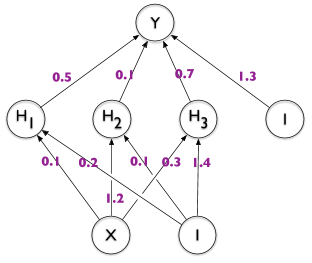
\includegraphics[width=1\columnwidth]{pres_pics/BNN_1}
		\end{figure}
	\end{minipage}
	\hfill
	\begin{minipage}[t]{0.47\columnwidth}
		\textbf{Bayesian Neural Networks} \\Predict the parameters of the weights distributions from the dataset
		\vspace{0.07cm}
		\begin{figure}
			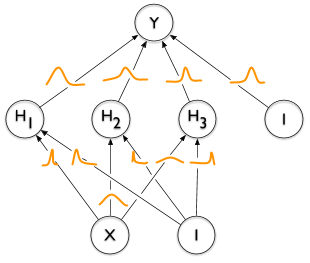
\includegraphics[width=1\columnwidth]{pres_pics/BNN_2}
		\end{figure}
	\end{minipage}
	\vfill
	\hrulefill
	
	\scriptsize{http://bit.ly/2rMQuDq}

\end{frame}
%--------------------------------------------------------------------------------
\begin{frame}{Deep Learning}
		\begin{figure}
			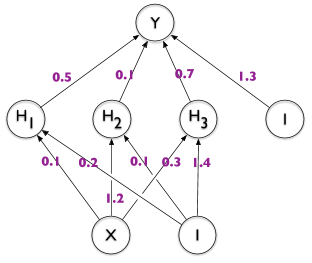
\includegraphics[width=1\columnwidth]{pres_pics/BNN_1}
		\end{figure}
		\begin{figure}
			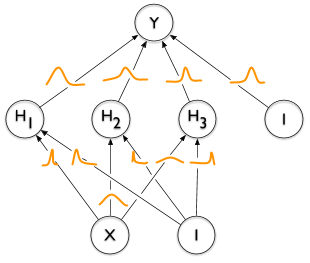
\includegraphics[width=1\columnwidth]{pres_pics/BNN_2}
		\end{figure}
	
\end{frame}
%--------------------------------------------------------------------------------
\begin{frame}{Experiments}
\begin{itemize}
	\item Synthetic datasets: moons, circles
	\item Real data: MNIST
\end{itemize}
Goals:
\begin{itemize}
	\item investigate influence of different priors on the predictions
	\item visualize uncertainties in predictions
	\item analyze the model behaviour
\end{itemize}
\end{frame}
%--------------------------------------------------------------------------------
\begin{frame}{Experiments}
	The best priors for moons and circles are gauss and cauchy with hyperprior respectively.
	\begin{columns}[t]
		\column{.5\textwidth}
		\centering
			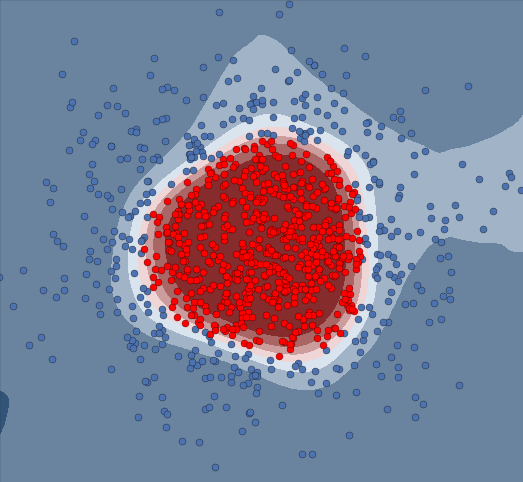
\includegraphics[width=4cm,height=3cm]{pres_pics/inv_cauchy_ppm.png}\ 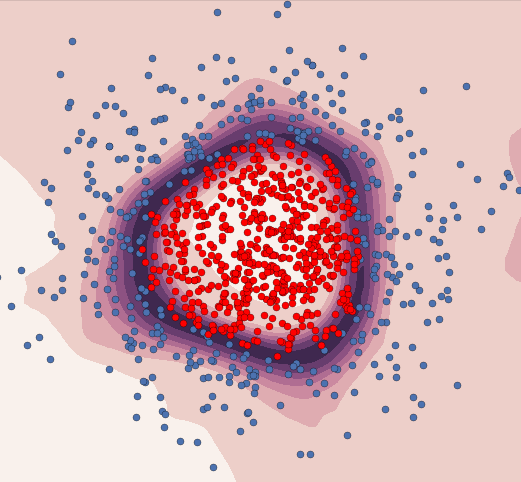
\includegraphics[width=4cm,height=3cm]{pres_pics/inv_cachy_uncert.png}
		\column{.5\textwidth}
		\centering
		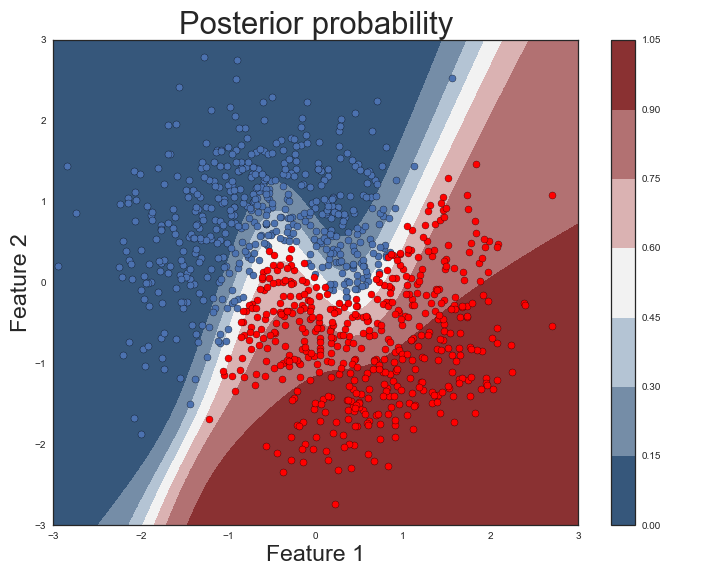
\includegraphics[width=4cm,height=3cm]{pres_pics/inv_gauss_ppm.png}\    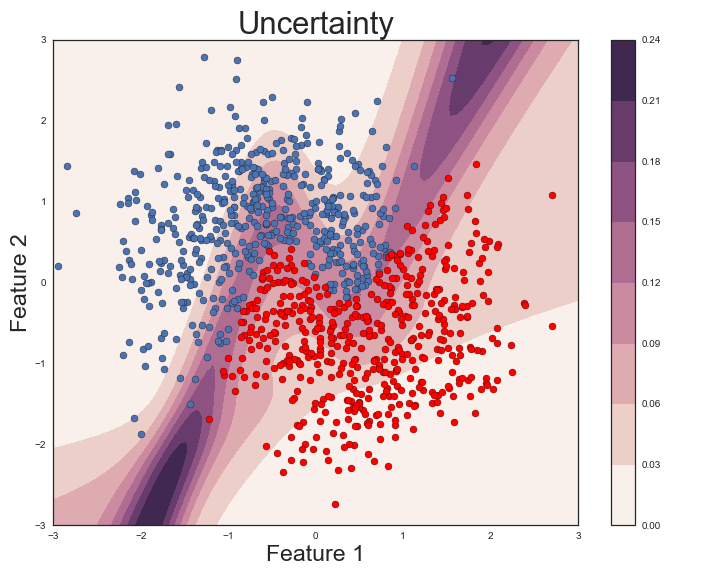
\includegraphics[width=4cm,height=3cm]{pres_pics/inv_gauss_uncert.png}
	\end{columns}
\end{frame}
%--------------------------------------------------------------------------------
\begin{frame}{Experiments}
	Including hyperpriors is almost always the best choice if we are unsure about prior parameters or data is noisy and hard.
	\begin{columns}[t]
		\column{.3\textwidth}
		\centering
		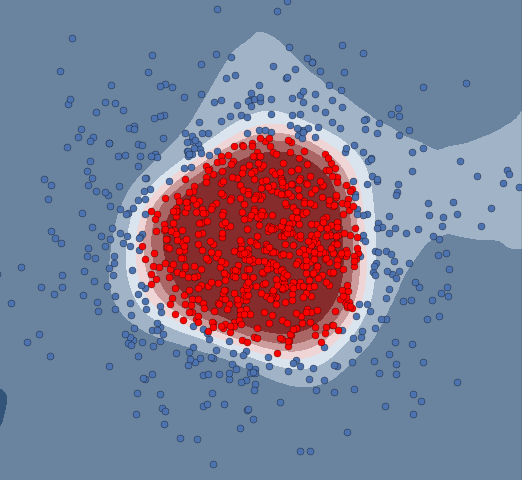
\includegraphics[width=4cm,height=3cm]{pres_pics/h_cauchy.png}\ 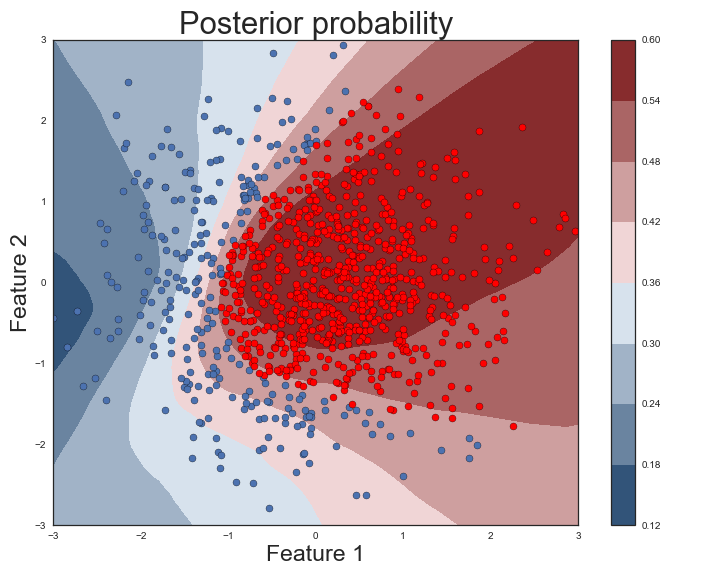
\includegraphics[width=4cm,height=3cm]{pres_pics/p_cauchy.png}
		\column{.3\textwidth}
		\centering
		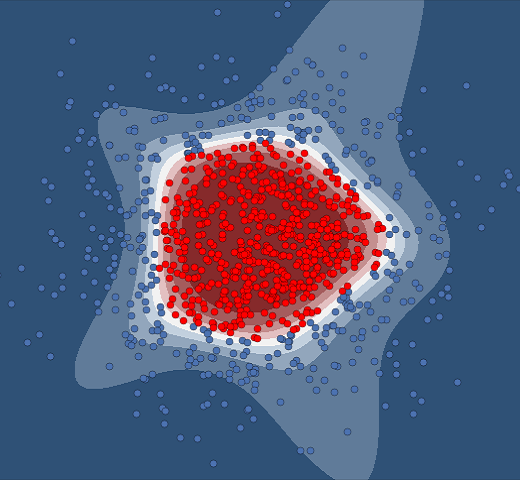
\includegraphics[width=4cm,height=3cm]{pres_pics/h_gauss.png}\    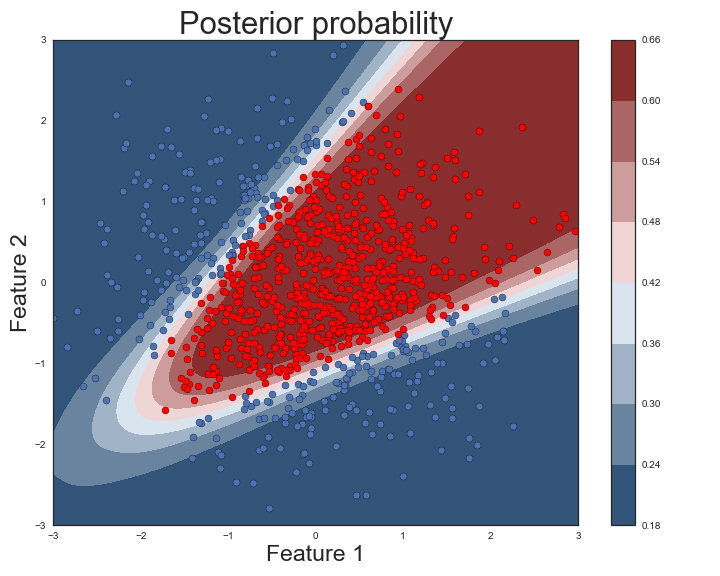
\includegraphics[width=4cm,height=3cm]{pres_pics/p_gauss.png}
		\column{.3\textwidth}
		\centering
		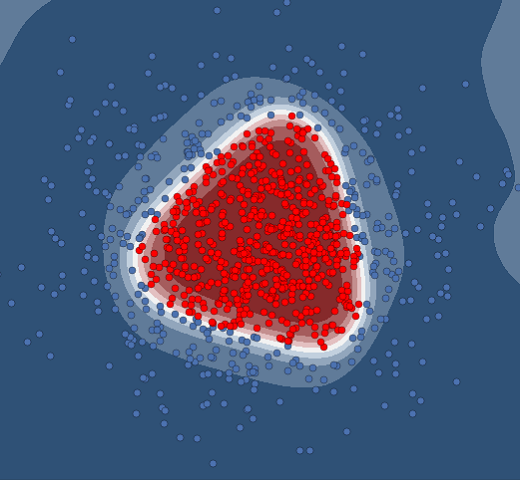
\includegraphics[width=4cm,height=3cm]{pres_pics/h_laplace.png}\    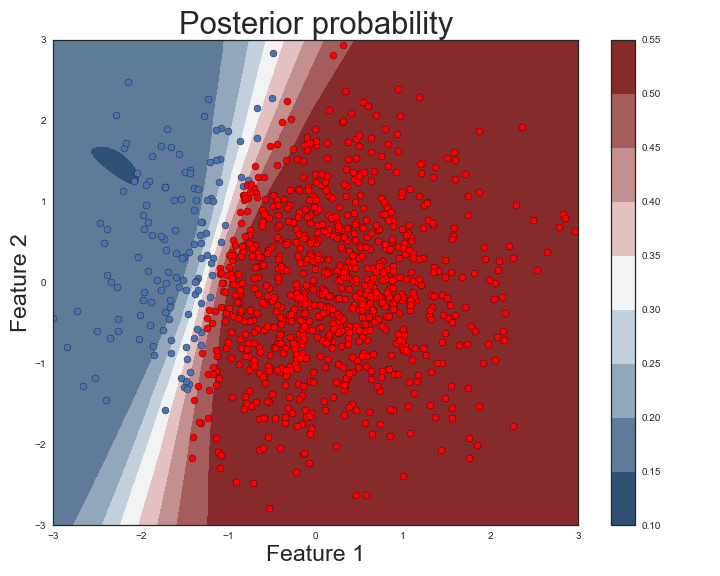
\includegraphics[width=4cm,height=3cm]{pres_pics/p_laplace.png}
	\end{columns}
\end{frame}

\begin{frame}{Experiments}
	Laplace prior does indeed provide sparser solutions compared to cauchy or gauss.
	\begin{columns}[t]
		\column{.5\textwidth}
		\centering
		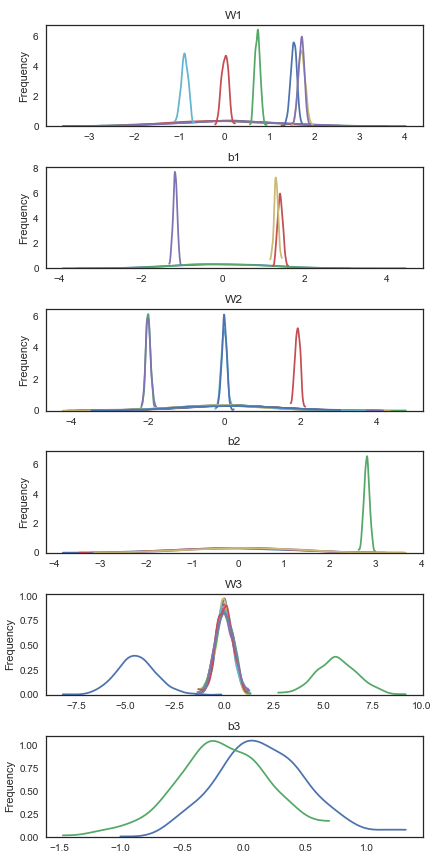
\includegraphics[width=4cm,height=7cm]{pres_pics/trace_laplace.png}
		\column{.5\textwidth}
		\centering
		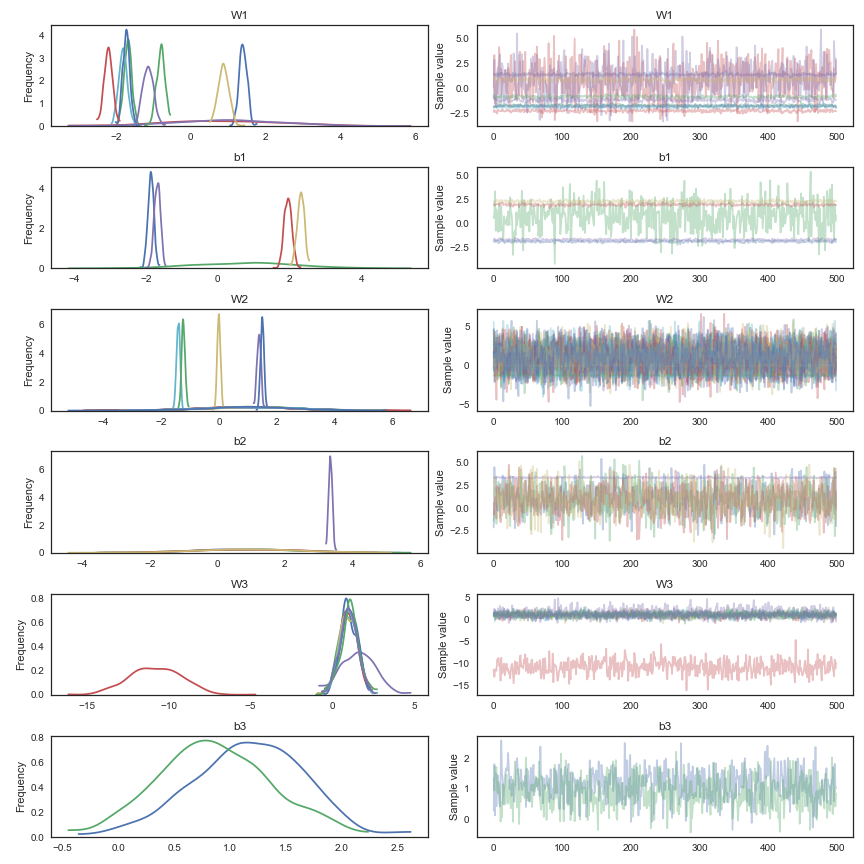
\includegraphics[width=4cm,height=7cm]{pres_pics/trace_cauchy.png}
	\end{columns}
\end{frame}


\end{document} 